\section{Lexer and parser generation}\label{sec:lexerandparsergen}
This section briefly covers how the lexer and parser for Arc has been implemented, and what alternatives could have been used.

The lexer, also called a lexical analyzer or scanner, takes a character stream and turns it into a list of tokens. Tokens are a representation of something in a language. A num in Arc would, for example, be a token that represents numbers. The lexer recognizes and can discard characters of the character stream, so that the parser can ignore them. For example is the parser not concerned with whitespaces, and nor does it need to, so it can simply discard them. If the lexer did not discard these, the parser would constantly have to check for them. These tokens are then passed on to the parser, which is tasked to make syntatic sense of them. It compares the tokens and their structure to the grammar of the specific language .

This section briefly covers the implementation of Arc's lexer and parser and available alternatives.

The lexer, also called a lexical analyzer or scanner takes a character stream and turns it into a list of tokens. Tokens are a representation of something in a language. A num in Arc would, for example, be a token that represents numbers. The lexer recognizes and can discard characters of the character stream so that the parser can ignore them. For example, is the parser not concerned with whitespaces, nor does it need to, so it can simply discard them. If the lexer did not discard these, the parser would constantly have to check for them. These tokens are then passed on to the parser, making syntactic sense of them. It compares the tokens and their structure to the grammar of the specific language~\cite{Parr2014}.

For Arc, \gls{antlr} has been used to describe the grammar and generate both the lexer and the parser. This choice made \gls{antlr} highly effective to work with when designing Arc, as minute changes to the grammar could easily be made without a worry - while the generation of the lexer and parser would not have to be recreated with every iteration~\cite{Parr2014}. Instead, only the grammar would ever need to be updated to reflect our changes, and then \gls{antlr}  would be responsible for generating all of the necessary files based on the new grammar.

The grammar was made in a file called 'arc.g4', an \gls{antlr} grammar file used to state the rules of the language. We decided to use a modular approach and segregate the lexer and parser rules into separate files. Therefore, the lexer rules are found in 'lexerRules.g4' and are imported into the main arc grammar file. These two files are everything \gls{antlr} needs to generate all needed files for the parser and the lexer.

Figure~\ref{fig:lexerandparserfiles} shows the files that \gls{antlr} generates when including the '-visitor' flag during compilation. The flag is responsible for generating the parse tree visitor files. The file 'arcLexer.java' is the lexer responsible for the lexical analysis, and the file 'arcParser.java' is the parser. Then there is a list of tokens for both grammar files and some other boilerplate code necessary for the analysis. Finally, the file 'arcVisitor.java' acts as the visitor interface, while the 'arcBaseVisitor.java' is the abstract class implementing the visitor interface. Most of these files are boilerplate and thus necessary for \gls{antlr} to work its magic. Much further detail about these files is beyond the scope of this project.


\begin{figure}[htb!]
    \begin{center}
        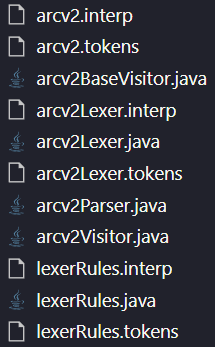
\includegraphics[width=0.25\textwidth]{figures/lexerAndParserFiles.png}
        \caption{Files generated for Arcs parser and lexical analyzer, including the flag '-visitor'}
        \label{fig:lexerandparserfiles}
    \end{center}
\end{figure}


Listing~\ref{lst:parserandlexerexample} shows how the parser, lexer, and visitor are used in practice. In line 1, an input is created from a text file. This input is a character stream used by the lexer instantiated in line 2. Then, a list of tokens is created based on the lexical analysis in line 3 and given to the parser in line 4. Now that the input has been parsed, the \gls{cst} is created in line 5 and is ready to be traversed in line 6, using our custom visitor class inheriting from the 'ArcBaseVisitor' class.


\begin{listing}[htb!]
    \begin{minted}{java}
        CharStream input = CharStreams.fromFileName("src/astTestFile.txt");
        arcLexer lexer = new arcLexer(input);
        CommonTokenStream tokens = new CommonTokenStream(lexer);
        arcParser parser = new arcParser(tokens);
        ParseTree tree = parser.start();
        // Any custom Visitor classes
    \end{minted}
    \caption{An example of how the parser and lexer is used}
    \label{lst:parserandlexerexample}
\end{listing}


We have learned a lot about parsers and lexers from the semester courses and from reviewing \gls{antlr}s generated files and documentation. Writing our own from scratch could also have been an enriching educational opportunity. Alas, this would also have meant considerably extra development time, while any potential changes also need to be reflected in all layers of the code. One small change to the grammar file would also have to be changed in both the lexer and the parser. Using \gls{antlr} to handle that has saved us time and energy so that we could focus on learning rather than maintaining a custom solution.